\documentclass[a4paper]{report}
\usepackage[spanish]{babel}
\selectlanguage{spanish}
\usepackage[utf8]{inputenc}
\usepackage[T1]{fontenc}
\usepackage{pdfpages}
\usepackage[a4paper,top=2cm,bottom=2cm,left=2cm,right=2cm]{geometry}
\usepackage{amsmath, amsthm, amsfonts}
\usepackage{graphicx}

\def\blankpage{%
      \clearpage%
      \thispagestyle{empty}%
      \addtocounter{page}{0}%
      \null%
      \clearpage}
    
\title{Desarrollo de la Lógica Proposicional y de Primer Orden bajo el paradigma funcional y la orientación Web.}
\author{Víctor Ramos González\\\\
   Tutor: Fernando Sancho Caparrini\\
   \textit{Ciencias de la Computación e Inteligencia Artificial}\\
   E.T.S. Ingeniería Informática\\
   Universidad de Sevilla\\
  \vspace{8cm}
  \date{Septiembre 2020}
}



\begin{document}

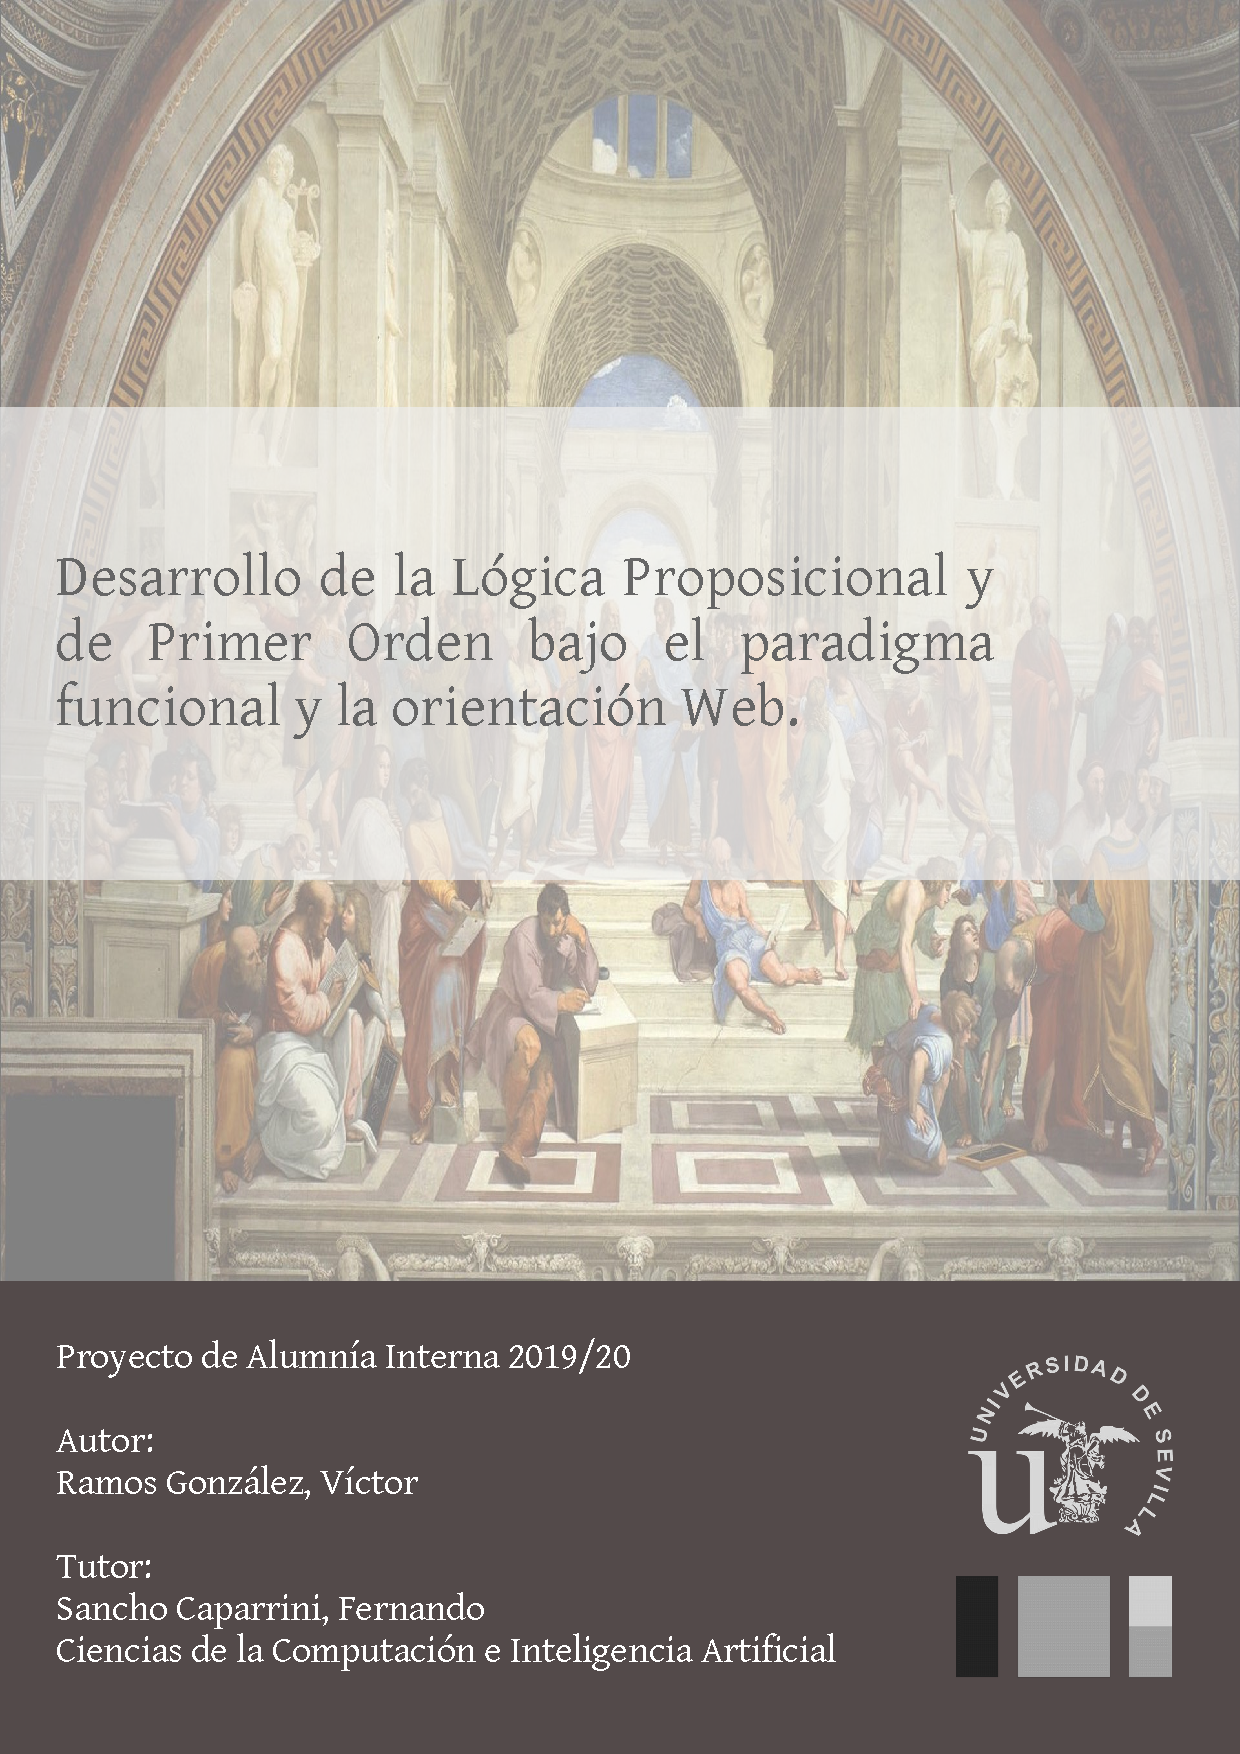
\includepdf[pages={1}]{archivos/titlepage.pdf}


\blankpage

\maketitle

\begin{abstract}

El proyecto aborda los conceptos y algoritmos básicos de la Lógica Proposicional y la Lógica de primer, desde un punto de vista implementativo a través de un lenguaje encuadrado en el paradigma funcional (Elm).\\

El proyecto, basado en la asignatura de Lógica Informática, busca una doble finalidad, por un lado servir como una somera introducción a la programación declarativa al mismo que tiempo que proporcionar al alumnado  herramientas intuitivas y de sencillo uso en la realización de los ejercicios que apoyen los contenidos teóricos que se desarrollan en dicha asignatura.\\
\end{abstract}

\tableofcontents

\newpage


\chapter{Introducción. Objetivos y organización del proyecto}
\chapter{LP I. Sintaxis y Semántica}
\chapter{LP II. Tableros Semánticos}
\chapter{LP III. Formas Normales y DPLL}
\chapter{LP IV. Sistemas Deductivos}
\chapter{LP V. Algoritmo de Resolución}
\chapter{LP VI. Modelado y Resolución de PSR a través de la LP}

\chapter{LPO I. Sintaxis y Semántica}
\chapter{LPO II. Tableros Semánticos}
\chapter{LPO III. Forma Prenex, Skolem y Teorema de Herbrand}
\chapter{LPO V. Algoritmos de Unificación y Resolución}
\chapter{LPO VI. Modelado y Resolución de PSR a través de la Lógica de Primer Orden}

\end{document}